\chapter{Domain Analysis}

% \instructions{
%     Describe the problem domain using a domain model as covered in the SEP1 module.
% }

To analyse KubeWatch's problem domain we use a domain model. We chose the domain model, because it allows us to have a common understanding of what the problem domain for \textit{KubeWatch} is, and how different components are connected to each other.

\section{Domain Model}
The different elements in our domain model (see figure \ref{fig:domain-model}) are the basis for our \hyperref[section:functional-requirements]{functional requirements} . If there are any further enhancements planned, which are outside the current scope, we will adjust and enhance the domain model accordingly.

\vspace{1cm}

\begin{figure}[h]
    \centering
    \caption{KubeWatch Domain Model}
    \label{fig:domain-model}
    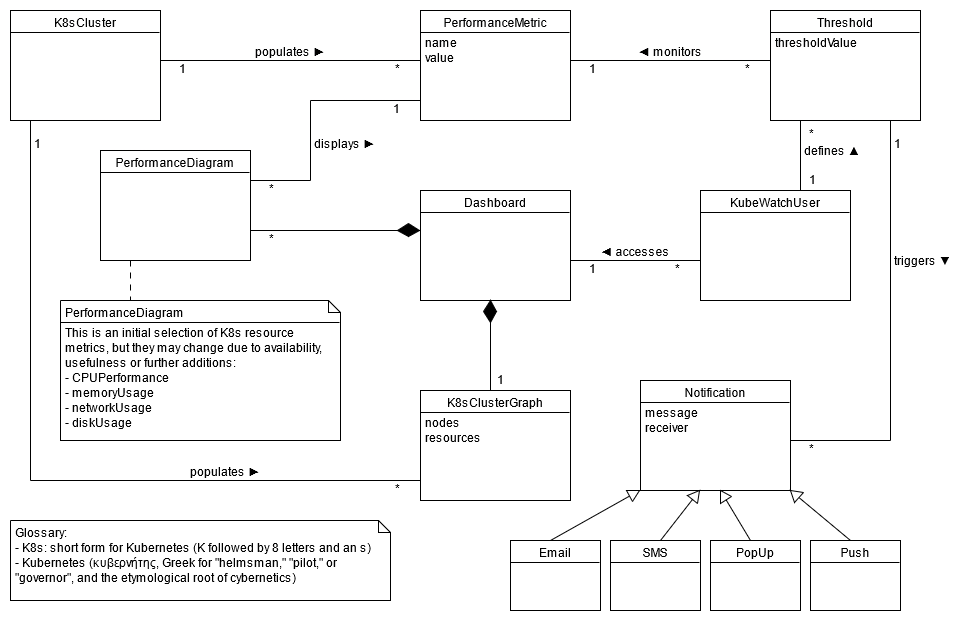
\includegraphics[width=\textwidth]{resources/domain_model.png}
\end{figure}